\NeedsTeXFormat{LaTeX2e}
%\PassOptionsToClass{handout}{beamer}
\documentclass{beamer}
\usepackage{beamerPack}
\usepackage[boxed,ruled,vlined]{algorithm2e}
\usepackage[03]{../lecture}
\subtitle{}
\begin{document}

\begin{frame}[fragile]{}
\titlepage
\end{frame}

\section{sort}		%%%%%%%%
\subsection{}

\begin{frame}[fragile]{整列}{}
\begin{itemize}\itemindent15mm\labelsep10mm
\item[初期状態]入力: 配列\texttt{VecT}

\medskip
\scalebox{0.6}{
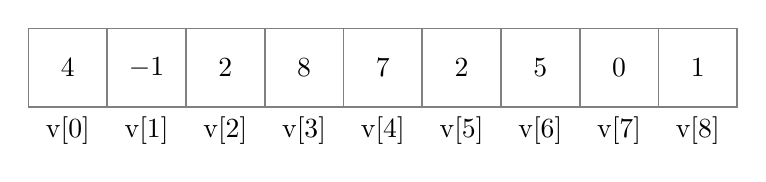
\begin{tikzpicture}[
    , cell/.style = {rectangle,draw=gray,semithick,minimum size=1cm,outer sep = 0mm,label=below:v{[\j]}}
]
\foreach \i [count=\j from 0] in {4, -1, 2, 8, 7, 2, 5, 0, 1}
    \node[cell] at (\j, 0) {$\i$};
\end{tikzpicture}
}
\item[最終状態]出力: 整列ずみの配列\texttt{VecT}

\medskip
\scalebox{0.6}{
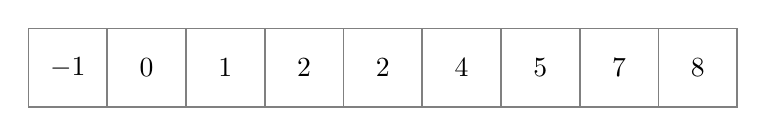
\begin{tikzpicture}[
    , cell/.style = {rectangle,draw=gray,semithick,minimum size=1cm,outer sep = 0mm}
]
\foreach \i [count=\j from 0] in {-1, 0, 1, 2, 2, 4, 5, 7, 8}
    \node[cell] at (\j, 0) {$\i$};
\end{tikzpicture}
}
\end{itemize}
全ての要素に順序がつけられること:全順序性が必要。
\vfill
\begin{block}{安定なソート}
順序が同じ要素は整列後も元の順序を保つ
\end{block}

氏名順に並んでいた学生データの配列を成績順にソート
\end{frame}

\section{bubble sort}		%%%%%%%%
\subsection{}

\begin{frame}[fragile]{bubble sort}{}
\scalebox{0.5}{
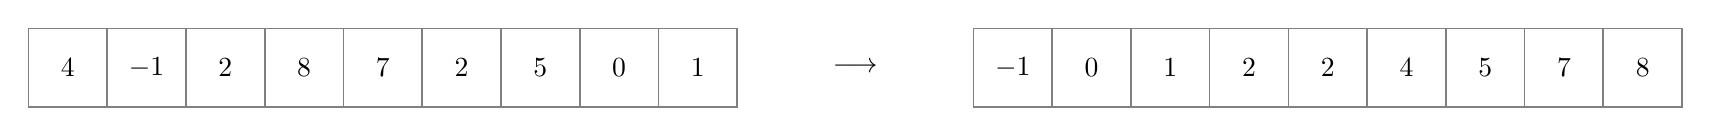
\begin{tikzpicture}[xshift=0.15\textwidth
    , cell/.style = {rectangle,draw=gray,semithick,minimum size=1cm,outer sep = 0mm}
]
\foreach \i [count=\j from 0] in {4, -1, 2, 8, 7, 2, 5, 0, 1}
    \node[cell] at (\j, 0) {$\i$};
\node at (10, 0) {$\longrightarrow$};
\foreach \i [count=\j from 0] in {-1, 0, 1, 2, 2, 4, 5, 7, 8}
    \node[cell] at (\j + 12, 0) {$\i$};
\end{tikzpicture}
}

\vfill
適切な中間目標を設定せよ

\pause
\vfill
先頭の1個が整列している

\vfill
\scalebox{0.6}{
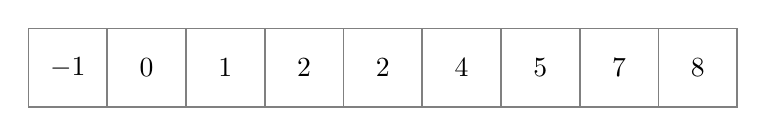
\begin{tikzpicture}[cell/.style = {rectangle,draw=gray,semithick,minimum size=1cm,outer sep = 0mm}]
\foreach \i [count=\j from 0] in {-1, 0, 1, 2, 2, 4, 5, 7, 8}
    \node[cell] at (\j, 0) {$\i$};
\end{tikzpicture}
}
{\tiny 中間目標になってない}

\medskip
\scalebox{0.6}{
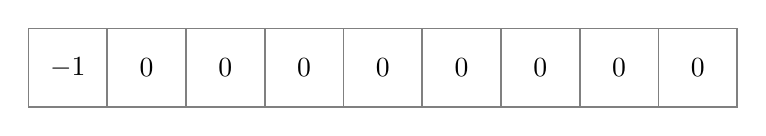
\begin{tikzpicture}[cell/.style = {rectangle,draw=gray,semithick,minimum size=1cm,outer sep = 0mm}]
\foreach \i [count=\j from 0] in {-1, 0, 0, 0, 0, 0, 0, 0, 0}
    \node[cell] at (\j, 0) {$\i$};
\end{tikzpicture}
}
{\tiny 次のステップにいけない}

\medskip
\scalebox{0.6}{
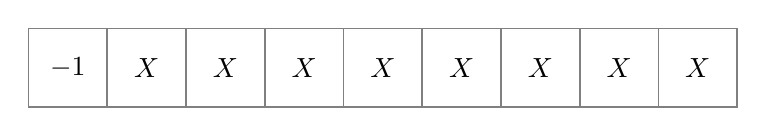
\begin{tikzpicture}[cell/.style = {rectangle,draw=gray,semithick,minimum size=1cm,outer sep = 0mm}]
\foreach \i [count=\j from 0] in {-1, X, X, X, X, X, X, X, X}
    \node[cell] at (\j, 0) {$\i$};
\end{tikzpicture}
}
{\tiny $X$は-1以外の要素のどれか}
\end{frame}

\begin{frame}[fragile]{bubble sort}{}

\begin{enumerate}%\itemsep8pt
\item
対象範囲$[0, N)$に対して、最も小さな要素を範囲の最初の位置に、それ以外の要素をそれ以降の範囲$[1, N)$に置く
\item
対象範囲$[1, N)$に対して、最も小さな要素を範囲の最初の位置に、それ以外の要素をそれ以降の範囲$[2, N)$に置く
\item
対象範囲$[2, N)$に対して、最も小さな要素を範囲の最初の位置に、それ以外の要素をそれ以降の範囲$[3, N)$に置く
\item
対象範囲$[N, N)$にはデータは存在しないので終了
\end{enumerate}
\end{frame}

\begin{frame}[fragile]{bubble sort}{}
\begin{algorithm}[H]
\KwIn{v: \texttt{Vec<T>}--対象配列}
\KwIn{start: Int -- 対象範囲の下限}
\KwIn{end: Int -- 対象範囲の上界}
\SetKwComment{Comment}{}{}
\BlankLine
i = 0\Comment*{\sl\small\color[gray]{0.5} 添字}
\While{i < end}{
  x = 範囲内で最も小さな要素(start, end)\;
  xとv[start]を入れ替え\;
  i += 1\;
}
\caption[page]{再帰を使わないアイデア}
\end{algorithm}

xだけでなくその添字も必要
\begin{itemize}%\itemsep8pt
\item 添字を返す
\item 最小値を返すのではなく、並び替えも途中でする
\end{itemize}
\end{frame}

\begin{frame}[fragile]{bubble sort in TypeScript}{}

\begin{codeof}{language=C}{bsort.ts}
function bsort<T>(v: Array<T>) {
  let last_index = v.length - 1
  for (let i = 0; 0 < last_index; i++) {
    for (let j = last_index; i < j; j--) {
      if (v[j] > v[j - 1]) {
        v[j]とv[j -1]を入れ替え // v.swap(j, j - 1)
      }
    }
  }
}
\end{codeof}
\end{frame}

\begin{frame}[fragile]{bubble sortの評価}{}
対象範囲$[0, N)$に対して、最も小さな要素を範囲の最初の位置に、それ以外の要素をそれ以降の範囲$[1, N)$に置く

対象範囲を変えて繰り返す
→範囲は1ずつ減る:N個のデータならN回繰り返し


対象範囲の中で最も小さな要素を範囲の最初の位置に置く
→対象範囲をrとするとこの操作は比較をr回繰り返す

\begin{align*}
最悪比較回数 &= N + (N - 1) + (N - 2) + (N - 3) + \cdots + 1 \\
&= \Sigma_{n=1}^{N}N \\
&= \frac{(N-1)N}{2} \\
&= \frac{1}{2}N^2 - \frac{1}{2}N \\
&= O(N^2)
\end{align*}

\end{frame}

\begin{frame}[fragile]{bubble sortの計算量評価}{}
a
\end{frame}

\section{quick sort}		%%%%%%%%
\subsection{}

\begin{frame}[fragile]{quick sort}{}
\scalebox{0.5}{
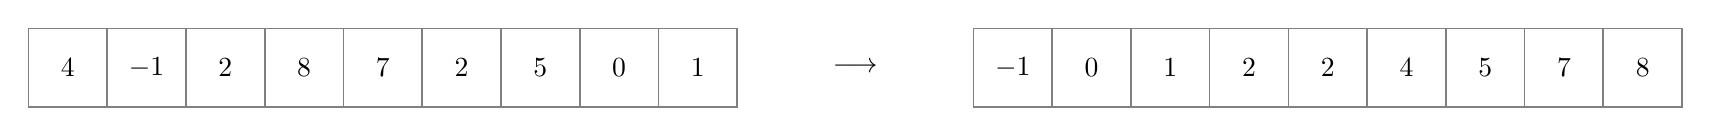
\begin{tikzpicture}[xshift=0.15\textwidth
    , cell/.style = {rectangle,draw=gray,semithick,minimum size=1cm,outer sep = 0mm}
]
\foreach \i [count=\j from 0] in {4, -1, 2, 8, 7, 2, 5, 0, 1}
    \node[cell] at (\j, 0) {$\i$};
\node at (10, 0) {$\longrightarrow$};
\foreach \i [count=\j from 0] in {-1, 0, 1, 2, 2, 4, 5, 7, 8}
    \node[cell] at (\j + 12, 0) {$\i$};
\end{tikzpicture}
}

\vfill
適切な中間目標を設定せよ

\pause
\vfill
N/2個のソート問題ふたつに帰着させる。

\begin{itemize}%\itemsep8pt
\item 他方のどの要素よりも小さい要素だけからなる配列
\item 他方のどの要素よりも大きい要素だけからなる配列
\end{itemize}
それぞれを整列、順につなげば全体が整列
\end{frame}

\begin{frame}[fragile]{quick sort in TypeScript}{}
\end{frame}

\begin{frame}[fragile]{quick sort in Rust/1}{}
\begin{codeof}{language=Rust}{quick sort}
/// v[beg..end]で最後の要素v[end - 1]以下の要素を[0..i]に移動
/// 注意:[b..e]はeを含まない(bは下限、eは上界)
fn partition<T: Ord>(v: &mut [T], beg: usize, end: usize) -> usize {
    let mut i = beg;
    for j in beg..end {
        if v[j] <= v[end - 1] {
            v.swap(i, j);
            i += 1;
        }
    }
    i
}
\end{codeof}
\end{frame}

\begin{frame}[fragile]{quick sort in Rust/2}{}
\begin{codeof}{language=Rust}{quick sort}
pub fn qsort<T: Ord>(v: &mut [T]) {
    sort(v, 0, v.len());
}

fn sort<T: Ord>(v: &mut [T], beg: usize, end: usize) {
    if beg + 1 >= end {
        return;
    }
    let p = partition(v, beg, end); // assert!(0 < end);
    sort(v, beg, p);
    sort(v, p, end);
}
\end{codeof}
\end{frame}

\begin{frame}[fragile]{quick sortの計算量評価}{最悪計算量、最良計算量、平均計算量}
a
\end{frame}

\begin{frame}[fragile]{quick sortの計算量評価}{前処理をした場合の最悪計算量}
\[
O(N)
\]
\end{frame}

\begin{frame}[fragile]{marginal caseへの対応}{}
\begin{codeof}{language=Rust}{quick sort}
fn partition<T: Ord>(v: &mut [T], beg: usize, end: usize) -> usize {
    let mut i = beg;
    for j in beg..end {
        if v[j] <= v[end - 1] {
            v.swap(i, j);
            i += 1;
        }
    }
    i.min(end - 1)
}
\end{codeof}

ループ終了時に$i = end$なら全ての要素がv[end-1]以下である。
これはv[end - 1]が最大値であることを意味する。
従って、次の範囲は[beg, end - 1]でよい。
\end{frame}

\section{summary}		%%%%%%%%
\subsection{}

\begin{frame}[fragile]{sortの比較}{}

{%\fontsize{9}{10}\selectfont
\begin{tabular}[h]{|l|r|r|r|}
\CH アルゴリズム & (最悪)時間--& 空間-- & 安定 \\
\CL バブルソート & $O(N^2)$ & $O(1)$ & ?\\
\CL クイックソート & $O(N\log(N))$ & $O(\log(N))$ & \\
\CL ヒープソート & $O(N\log(N))$ & $O(\log(N))$ & \checkmark \\
\CL マージソート & $O(N\log(N))$ & $O(\log(N))$ & \checkmark \\
\end{tabular}
}

\vfill
クイックソートは$O(N^2)$では? $O(N)$の前処理でほぼ対応できる。
\end{frame}

\begin{frame}[fragile]{ヒープソート}{}
データ構造ヒープにデータを登録、ヒープから整列されて出力

安定ソート
\vfill
追加の処理をしなくても最悪時間計算量は$O(N\log(N))$
\end{frame}

\begin{frame}[fragile]{マージソート}{}
データを二分。再帰的に処理して整列する、それぞれストリームとみなして一つに整流。

安定ソート

\vfill
追加の処理をしなくても最悪時間計算量は$O(N\log(N))$
\end{frame}

\begin{frame}[fragile]{追補}{}
\begin{itemize}\itemsep8pt
\item 多くの言語で標準ライブラリ化。多くの場合クイックソート、ただし各種改良が導入されている
\begin{itemize}%\itemsep8pt
\item 要素数が極めて少ない時はバブルソートを使う
\item スタックの消費を嫌って途中からヒープソート(キャッシュのヒット率??)
\end{itemize}
\vfill 上位N個までのソートが欲しい。言語によっては提供
\item 安定版、非安定版も言語によっては両方提供。
\end{itemize}
\end{frame}

\begin{frame}[fragile]{Summany}{}
\begin{itemize}%\itemsep8pt
\item 中間目標の設定・理解がアルゴリズム設計・高速化において重要
\item 問題の持つ帰納的構造を再帰的構造を持つプログラムに転移
\end{itemize}
\end{frame}

\end{document}
